\documentclass[crop=false]{standalone}
\begin{document}
	\section{System Overview}
	
	The system architecture, as shown in Figure 1, begins with RGBD cameras capturing images with depth information. These RGB and depth images are then fed into the YOLO object detection model. The object detection task is performed by a deep learning model, which detects objects and provides their positions. These positions are then transformed into coordinates and used by the DWA for dynamic path adjustment. Additionally, a shortest path algorithm is incorporated to enhance the speed of path selection in DWA. This shortest path allows the drone to reach the specified location in minimal time while avoiding obstacles.

	\begin{figure*}[thbp!]
		\centering
		\fbox{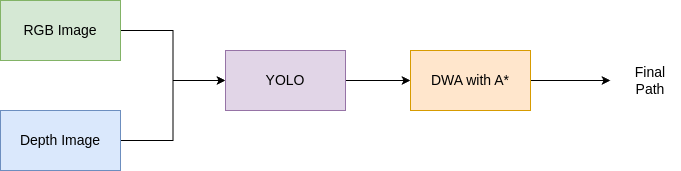
\includegraphics[width=\textwidth]{furtherwork_workflow}}
		\caption{The system architecture}
		\label{fig:system}
	\end{figure*}
\end{document}